\chapter{The Super Kamiokande Detector}
\label{chp:superk}


\section{Event Reconstruction}

\subsection{Vertex Reconstruction}
For low energy events (events up to 100MeV), Super-Kamiokande currently uses BONSAI (Branch Optimisation Navigating Successive Annealing Interactions) for event reconstruction. Vertex reconstruction for Super-Kamiokande has undergone changes and improvements depending on the phase of the experiment. 
\newline{}
For Phase I of Super-Kamiokande, vertex reconstruction depended on a lattice of test vertices with 4m spacing throughout the detector, with a specific measure of goodness for each test vertex: the test vertex with the highest measure of goodness would have around it a more finely spaced grid, and the process would be repeated. For Phase II of Super-Kamiokande due to the reduced number of PMTs, this approach was no longer as successful as it was in Phase I and as a result the reconstruction perfomance declined, and BONSAI was created as a replacement. Instead of using a fixed grid which was the case with SK-I and SK-II, BONSAI creates test vertices by selecting groups of four PMT hits and seeing where the timing residuals of the PMT hits would be most reduced. After these test vertices have been indentified, a maximum likelihood fit over all the PMT hits in the event is performed, shown in Equation \ref{bonsailikelihood}.

\begin{equation}
    \mathcal{L}(\vec{x}, t_{0})=\sum_{i=1}^{N_{\text {hlt }}} \log (P(t-t_{\text {tof }}-t_{0}))
\label{bonsailikelihood}
\end{equation}

where ($\vec{x}, t_{0}$) is the test vertex, and $(P(t-t_{\text {tof }}-t_{0}))$ is the probablility density function of the timing residual, which for each PMT hit is defined as $(t-t_{\text {tof }}-t_{0})$, where $t_{0}$ is the time of the interaction, $t_{tof}$ is the time of flight from the interaction vertex position to the position of the hit PMT, $t$ is the PMT hit time. The vertex resolution 

\begin{figure}
    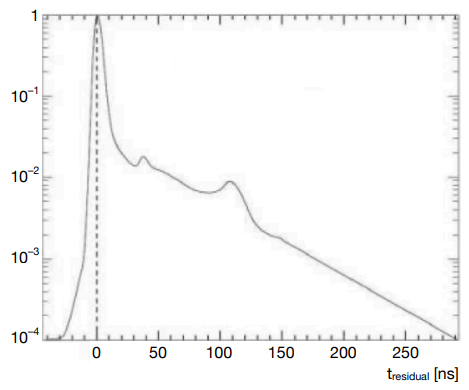
\includegraphics[scale=0.4]{Figures/bonsai_pdf_res.png}
\caption{Probability density of the timing residual P$(t-t_{\text {tof }}-t_{0})$, where $t_{0}$ use for the vertex reconstruction maximum likelihood fit. The peaks at 30ns and 100ns are caused by PMT after-pulsing. Figure from \cite[nakanopdf].}
    \label{bonsaivertexpdf}
\end{figure}

\begin{figure}
    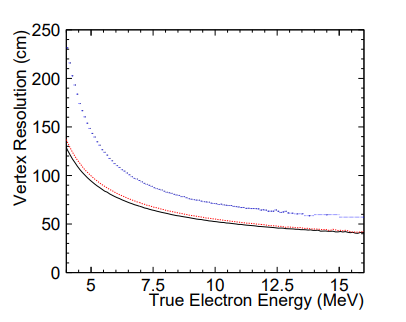
\includegraphics[scale=0.4]{Figures/bonsai_vertex_res.png}
\caption{The vertex resolution (the point at which 68\% of the events in the distance distribution between the actual and reconstructed vertex are contained) for the different SK phases. SK-I (Blue), SK-III (Red), SK-IV (Black).  Figure from \cite[nakanopdf].}
    \label{bonsaivertexres}
\end{figure}

\subsection{Direction Reconstruction}

Cherenkov light is emitted in a conical formation as electrons and positrons travel through water, with a Cherenkov angle of $\approx 42\degree$. BONSAI can reconstruct the direction of these particles by using this information along with the reconstructed vertex. This reconstruction occurs using a maximum likelihood function defined in Equation \ref{directionlikelihoodeq}.

\begin{equation}
    \mathcal{L}(\vec{d})=\sum_{i}^{N_{20}} \log (f(\cos\theta_{i}, E))\times\frac{\cos\theta_{i}}{a(\theta_{i})}
    \label{directionlikelihoodeq}
\end{equation}

$f(\cos\theta_{i},E)$ is the expected distribution of the angle between the vector of the direction $\vec{d}$ of the particle, and the observed Cherenkov photon from the position of the reconstructed vertex. The reason there is a spread in this energy distribution is because while the highest value of this distribution occurs at the cosine of the opening Cherenkov angle of $42\degree$, due to the particle travelling through the water being Coulomb scattered multiple times, there is a variation in the angle because of the varying particle energy. $N_{20}$ is the number of hits whose residual hit time is within 20ns of the time of the reconstructed event, which is used in order to reduce the amount dark noise and scattered photons contribute to the direction reconstruction calculation. The  variable $a(\theta_{i})$ is used in the second term in Equation \ref{directionlikelihoodeq}, and it is linked to the angle of incidence of the photon on the PMT $a(\theta_{i})$, and is a correction factor stemming from the acceptance of PMTs and therefore linked to the shape of the PMT and it's acrylic case. 


\subsection{Energy reconstruction}

The kinetic energy of a particle is proprtional to the amount of Cherenkov photons emitted from it, and if we assume that the Cherenkov photons in a single event come from a single electron, we can reconstruct the total energy of the electron. Instead of using the number of photoelectrons of all hit photomultiplier tubes to reconstruct the energy of low energy events, the number of hit photomultiplier tubes is used instead. The reasons for this are threefold - firstly, low energy events emit a small number of Cherenkov photons, and therefore average about one photon per hit PMT. Secondly, at single photoelectron level, the resolution of photoelectrons is bad, and third, the number of photoelectrons produced is related to the gain of the photomultiplier tubes, which is given by equation:

\begin{equation}
    G(i) \propto \frac{Q_{o b s}(i)}{N_{o b s}(i)}
\label{gain_equation}
\end{equation}

where $G(i)$ is the gain of each PMT and $Q_{obs}(i)$ is the average charge for each inner detector photomultiplier tube, and $N_{obs}(i)$ is the number of times that photomultiplier tube $i$ registers a charge which is greater than the threshold charge value. Due to the variation in gain value not affecting the number of hit photomultiplier tubes as much as it does for the number of photoelectrons, number of hit PMTs is used instead. Energy reconstruction uses $N_{50}$, which is the number of photomultiplier tube hits in a 50 ns window, which allows for the rejection of dark noise hits for the photomultiplier tubes. The number of effective photomultiplier tubes which are hit, the number of hit PMTs in this timing window of 50ns is summed up, while being weighted with correction factors, shown in Equation \ref{effectivePMTs}. 

\begin{equation}
    N_{e f f}=\sum_{i=1}^{N_{50}}\left[\left(X_{i}-\epsilon_{\text {dark }}+\epsilon_{\text {tail }}\right) \times \frac{N_{\text {all }}}{N_{\text {alive }}} \times \frac{1}{S\left(\theta_{i}, \phi_{i}\right)} \times \exp \left(\frac{r_{i}}{\lambda}\right) \times G(i)\right]
    \label{neff}
\end{equation}

where $X_{i}$ is the correction factor hits with many photoelectrons. This correction factor is important because if some photomultiplier tubes are hit by multiple photons (for example, if the edge of the fiducial volume is where the event vertex took place). The number of photoelectrons produced by each hit photomultiplier tube is estimated using the occupancy of the eight photomultiplier tubes which surround it. Using the number of hit photomultiplier tubes ($n_{i}$) and the number of functional photomultiplier tubes that surround the i-th photomultiplier tube ($N_{i}$), the formula for $X_{i}$ is shown in Equation \ref{correction_factor}.

\begin{equation}
    X_{i}=\left\{\begin{array}{ll}
        \log \left(1-n_{i} / N_{i}\right)^{-N_{i} / n_{i}} & \left(n_{i}<N_{i}\right) \\
        3 & \left(n_{i}=N_{i}\right)
        \end{array}\right.
        \label{correction_factor}
\end{equation}


$\epsilon_{dark}$ in Equation \ref{neff} is a correction factor for dark noise hits, shown in Equation \ref{edark}, where $R_{dark}$ is the average value for the dark rate during the run period that the event is in and $N_{\text {PMT}\text {alive }$ is the number of active photomultiplier tubes in the inner detector.


\begin{equation}
    \epsilon_{\text {dark }}=\frac{N_{\text {PMT}\text {alive }} \times R_{\text {dark }} \times 50 \mathrm{~ns}}{N_{50}}
    \label{edark}
\end{equation}

$\epsilon_{tail}$ is the correction factor for photomultiplier tube hits which are in the tail end of the 50ns timing window, and is defined in Equation $\ref{etail}$.

\begin{equation}
    \epsilon_{\text {tail }}=\frac{N_{100}-N_{50}-N_{\text {alive }} \times R_{\text {dark }} \times(100-50) \mathrm{ns}}{N_{50}}
    \label{etail}
\end{equation}

\frac{N_{all}}{N_{alive}} is the factor which corrects the time variation of the number of dead photomultiplier tubes, where $\N_{all}$ is equal to 11129, the total number of photomultiplier tubes in the inner detector of Super-Kamiokande. 

$\frac{1}{S\left(\theta_{i}, \phi_{i}\right)}$ is the inverse of the effective area of the ith hit photomultiplier tube photocathode, from the direction of the incident photon given by $(\theta_{i}, \phi_{i}\right)$.

$G(i)$ is the gain correction for the quantum efficiency of the photomultiplier tubes and $exp(\frac{r_{s}}{\lambda})$ is the correction for water transparency which accounts for the amount of attenuation undergone by the photons in water, where $\lambda$ is the water transparency measured during the run period which includes the event, and $r_{i}$ is the distance between the reconstructed event vertex and the i-th hit PMT.

